%%%%%%%%%%%%%%%%%%%%%%%%%%%%%%%%%%%%%%%%%
% Memo
% LaTeX Template
% Version 1.0 (30/12/13)
%
% This template has been downloaded from:
% http://www.LaTeXTemplates.com
%
% Original author:
% Rob Oakes (http://www.oak-tree.us) with modifications by:
% Vel (vel@latextemplates.com)
%
% License:
% CC BY-NC-SA 3.0 (http://creativecommons.org/licenses/by-nc-sa/3.0/)
%
%%%%%%%%%%%%%%%%%%%%%%%%%%%%%%%%%%%%%%%%%

\documentclass[letterpaper,11pt]{texMemo} % Set the paper size (letterpaper, a4paper, etc) and font size (10pt, 11pt or 12pt)

\usepackage{parskip} % Adds spacing between paragraphs
\usepackage{hyperref}
\frenchspacing
\setlength{\parindent}{15pt} % Indent paragraphs

\hypersetup{colorlinks=true, urlcolor=blue, citecolor=black, linkcolor=blue}

%----------------------------------------------------------------------------------------
%	MEMO INFORMATION
%----------------------------------------------------------------------------------------

\memoto{NFPA 1961 Technical Committee} % Recipient(s)

\memofrom{NIST Firefighting Technology Group} % Sender(s)

\memosubject{Full-scale Exposure Testing of Hoselines} % Memo subject

\memodate{\today} % Date, set to \today for automatically printing todays date

%----------------------------------------------------------------------------------------

\begin{document}

\maketitle % Print the memo header information

%----------------------------------------------------------------------------------------
%	MEMO CONTENT
%----------------------------------------------------------------------------------------

This letter report documents two experiments performed at the request of NFPA staff for use by the NFPA Technical Committee on Fire Hose.   The objective of the experiments was to gain some insight into the failure of fire hose as a result of thermal insult.  Three different hose conditions were examined; hose filled with air, hose filled with water, hose flowing 150~gpm of water. 

\section{Experimental Test Arrangement}
The experiments were conducted in a two story structure that was built to simulate a townhouse with a walk out basement. The structure was built on a concrete slab. The lower level of the structure had an outer wall composed of 0.6~m (2~ft) thick interlocking concrete blocks. The joints and gaps between the blocks were filled with high temperature foam insulation. The interior walls of the lower level were framed with steel studs and track. The studs were set to 0.40~m (16~in.) centers. The ceiling/floor support was composed of wood truss joist I-beams (TJIs) with a 299~mm (11.75~in.) depth. Each TJI was composed of laminated veneer lumber flanges with a cross section of 29~mm (1.13~in.) x 44~mm (1.75~in.) and an 11~mm (0.43~in.) thick oriented strand board web. Tongue and grove, 18.3~mm (0.72~in.) thick, oriented strand board was screwed to the top of the TJIs to form the floor of the upper level. The walls and ceiling of the lower level was composed of two layers of 12.7~mm (0.5~in.) thick cement board. 

The upper level of the structure was built on the wood floor assembly above. The walls were framed with wood studs set to 0.40~m (16~in.) centers. The walls and ceiling of the upper level were composed of two layers of 12.7~mm (0.5~in.) thick cement board.   

The interior footprint of the lower level is approximately 5.7~m (18.7~ft) wide by 10.6~m (34.8~ft) deep. The interior area of the upper level is approximately 6.0~m (19.8~ft) wide by 11~m (36~ft) deep.	 Figures~\ref{fig:schematic_low} and \ref{fig:schematic_up} are schematics of the floor plans of the upper and lower levels. In these images, circles indicate the location of thermocouples, squares indicate the location of velocity probes and thermocouples, diamonds indicate gas measurement probes, and triangles indicate the location of heat flux measurements.

\begin{figure}[!ht]
\centering
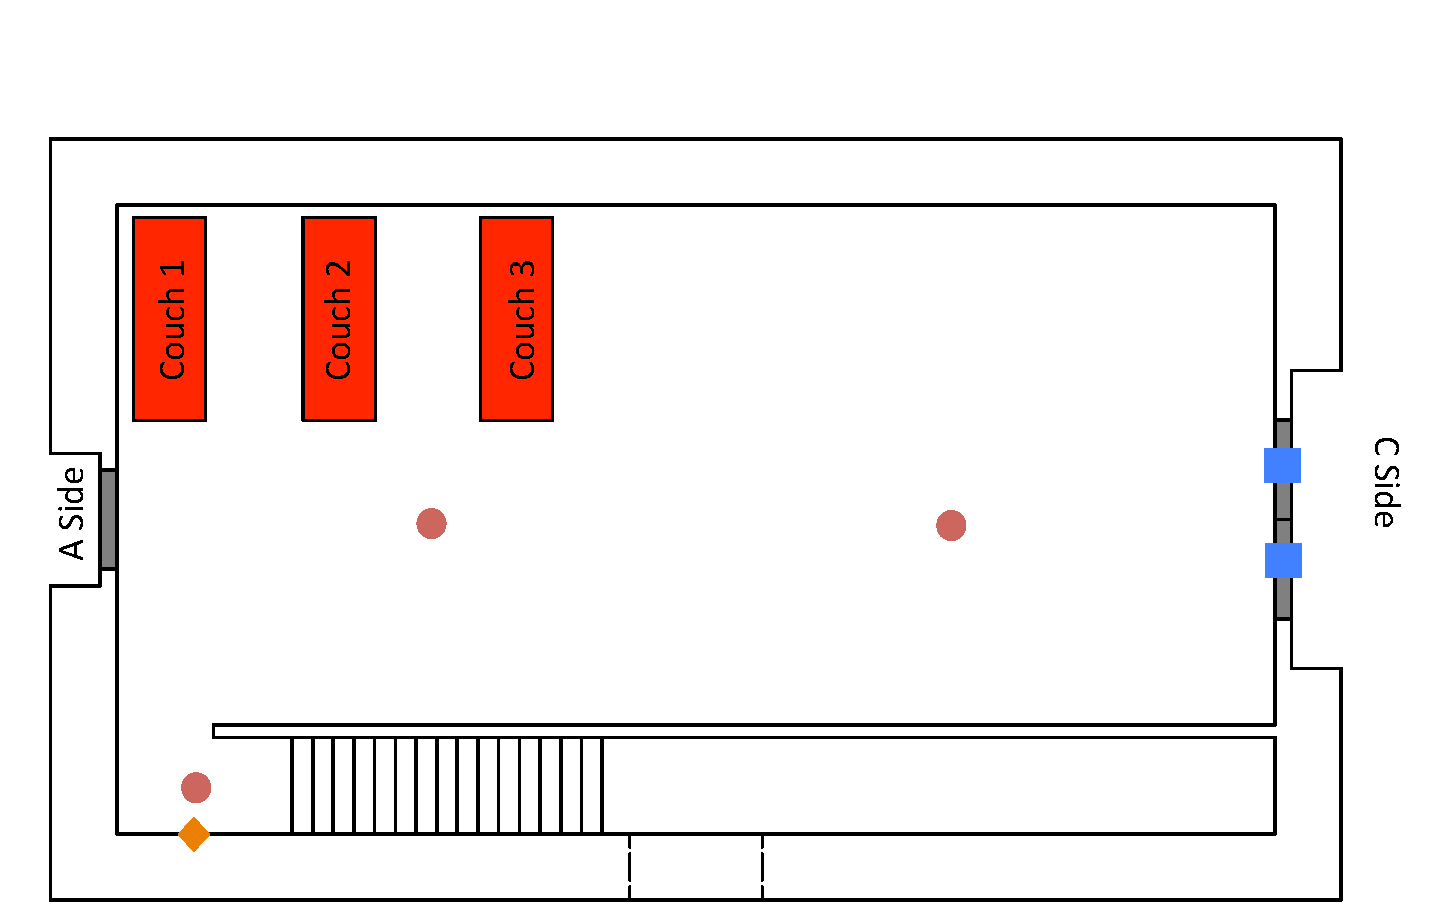
\includegraphics[width=0.8\columnwidth]{../Figures/Hose_Figures/schematic_lower}
\caption{Schematic of Lower Level}
\label{fig:schematic_low}
\end{figure}

\begin{figure}[!ht]
\centering
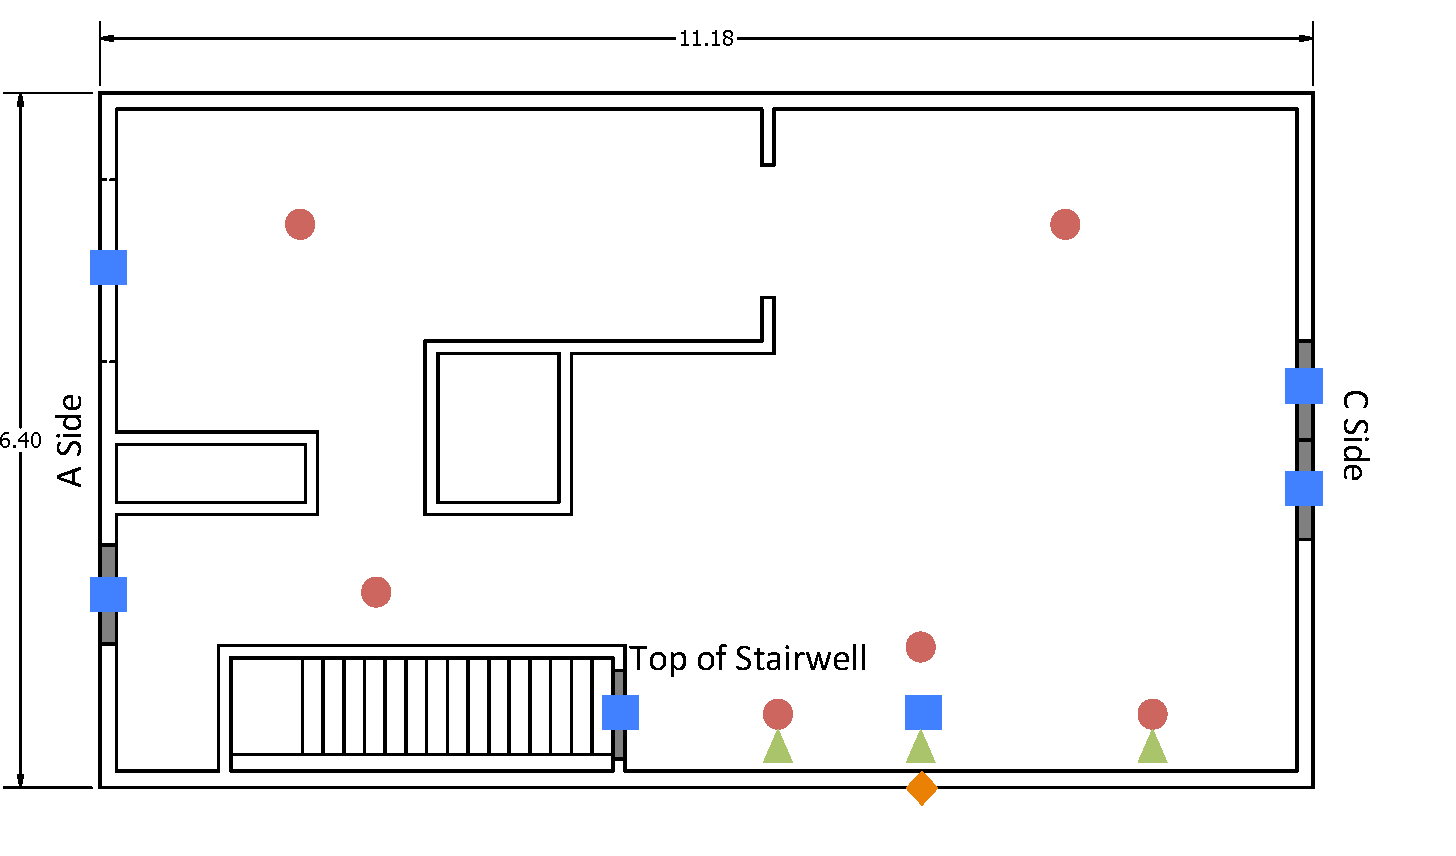
\includegraphics[width=0.8\columnwidth]{../Figures/Hose_Figures/schematic_upper}
\caption{Schematic of Upper Level}
\label{fig:schematic_up}
\end{figure}

On Side C of the lower level, there is a set of doors with a total opening of approximately 1.8~m (6~ft) wide and 2.0~m (6.7~ft) high. These doors were open for the duration of the hose exposure experiments.  

On Side A of the lower level the single door remained closed for these experiments. The door was undercut to allow the hoses to pass through without any obstruction. Non-combustible fiber was then packed around the hoses to minimize any leakage under the door.  An open stair extends from Side A and leads to the upper level with an open doorway facing Side C of the structure. The ventilation openings on the upper level include a 36~in. by 80~in. doorway and a 66~in. wide by 36~in. high window with a 43~in. sill height on the A side. On C side of the upper level is another set of double doors similar in size to the set of doors on the lower level. All of the openings on the upper level remained closed for the duration of the hose exposure experiments. See schematics of the floor plans (Fig.~\ref{fig:schematic_low} and \ref{fig:schematic_up}) of both levels and photographs of the exterior of the structure (cf. Fig.~\ref{fig:exterior}).

\begin{figure}[!ht]
\centering
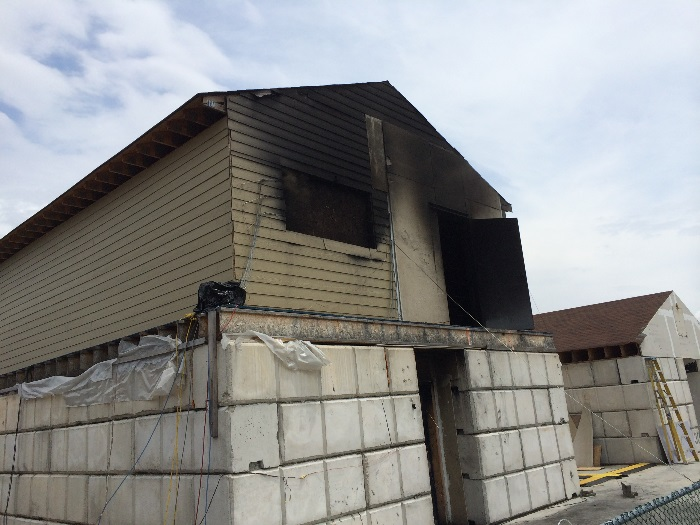
\includegraphics[width=0.45\columnwidth]{../Figures/Hose_Figures/exterior_a}
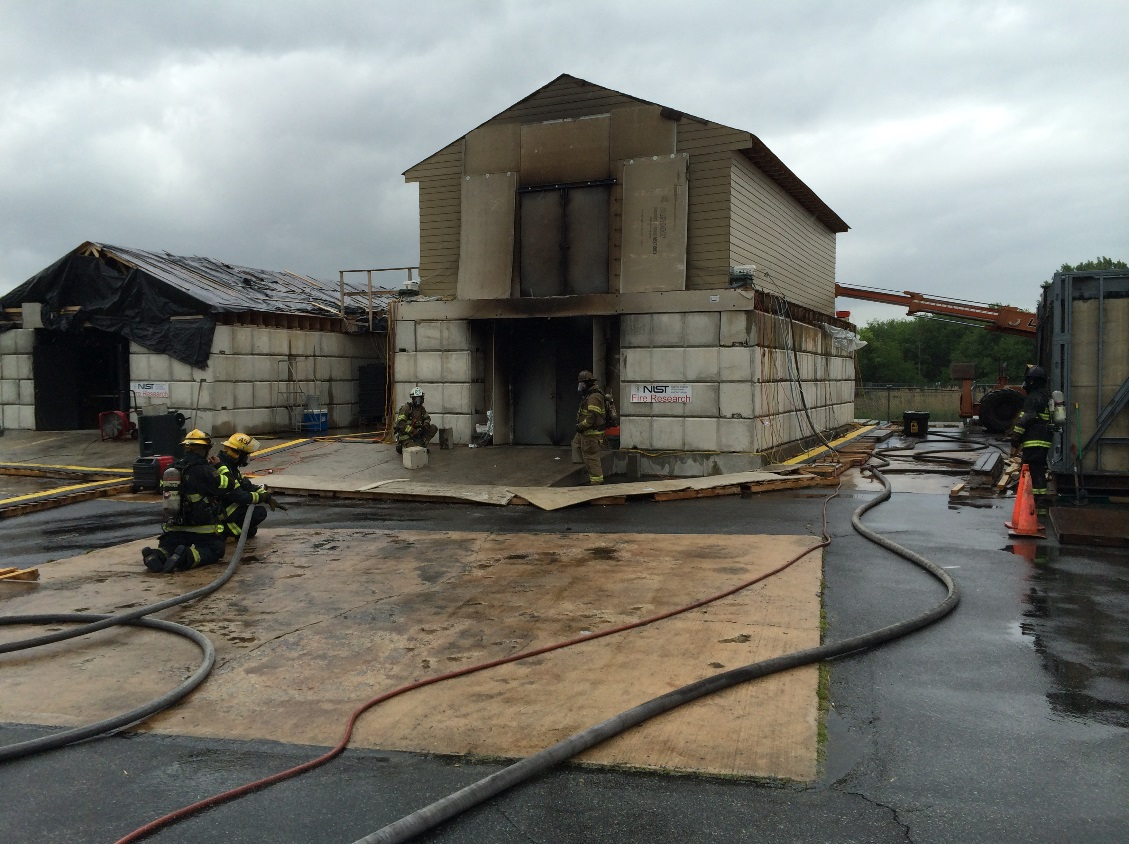
\includegraphics[width=0.45\columnwidth]{../Figures/Hose_Figures/exterior_c}
\caption{Photographs of Side A (Left) and Side C (Right). }
\label{fig:exterior}
\end{figure}

\section{Fuel Load}
The interior finish of the lower level consisted of 12.7~mm (1/2~in.) oriented strand board (OSB).  The OSB covered the entire ceiling, floor and the walls on Sides A, B, and D. Polyolefin carpeting over polyurethane foam padding covered the floor of the lower level.  The fuel load in the basement consisted of three sofas, oriented strand board on the ceiling and walls of the basement (cf. Fig.~\ref{fig:schematic_low}).  In a free burn condition, each sofa can generate a peak heat release rate of approximately 2~MW.

\section{Instrumentation}
Temperatures were measured with bare-bead, Chromel-Alumel (type K) thermocouples, with a 0.5~mm (0.02 in) nominal diameter. A vertical thermocouple array was installed adjacent to the center of the test section of the hoses on the floor of the lower level. The vertical array had thermocouples located 0.025, 0.3, 0.61, 0.91, 1.22, 1.52, 1.83, 2.13~m (1~in., 1,2,3,4,5,6,7 ft.) below the ceiling (BC).  Additional single thermocouples were installed in contact with the outer jacket of the fire hoses.  

The heat flux gauges used were Schmidt-Boelter type, water cooled gauges.  Total heat flux, convection and radiation, was measured with the uncovered gauge. Radiant heat flux was measured with a gauge covered with a sapphire lens.  

\begin{figure}[!ht]
\centering
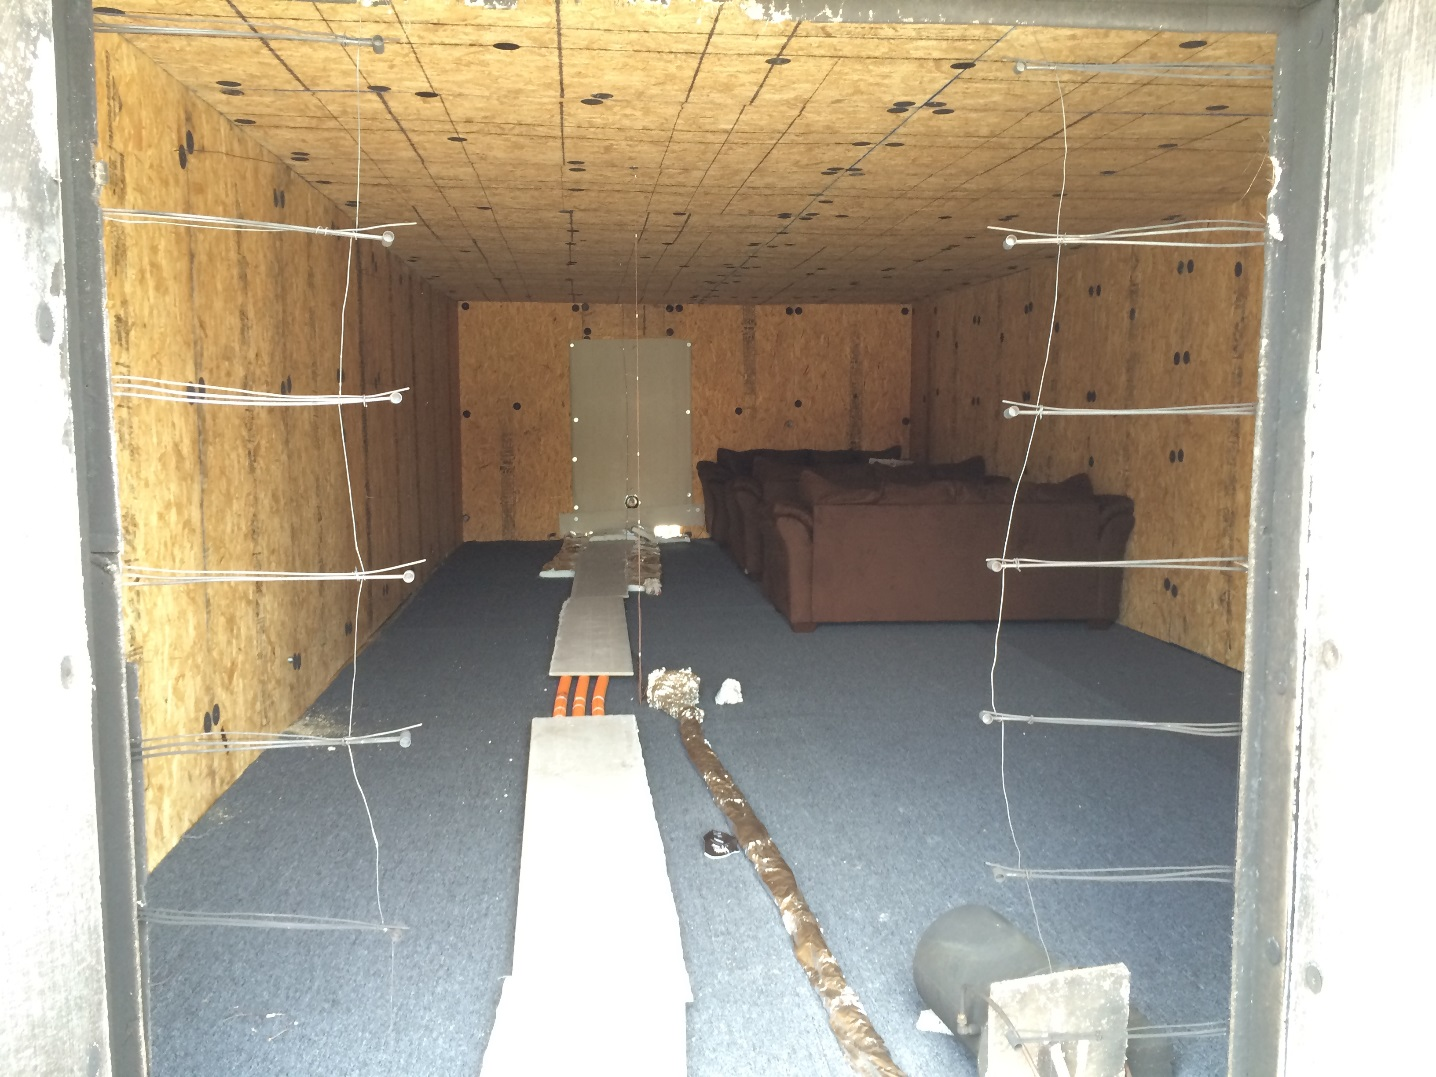
\includegraphics[width=0.8\columnwidth]{../Figures/Hose_Figures/test_setup_1}
\caption{Fire room with fuel load, instrumentation and hose samples installed for Experiment 1. Looking in from the Side C open doorway on the lower level. These doors are the only opening in the structure during the test. As a result the fire will move from the back of the room over the exposed hose toward the door.}
\label{fig:test_setup_1}
\end{figure}

\begin{figure}[!ht]
\centering
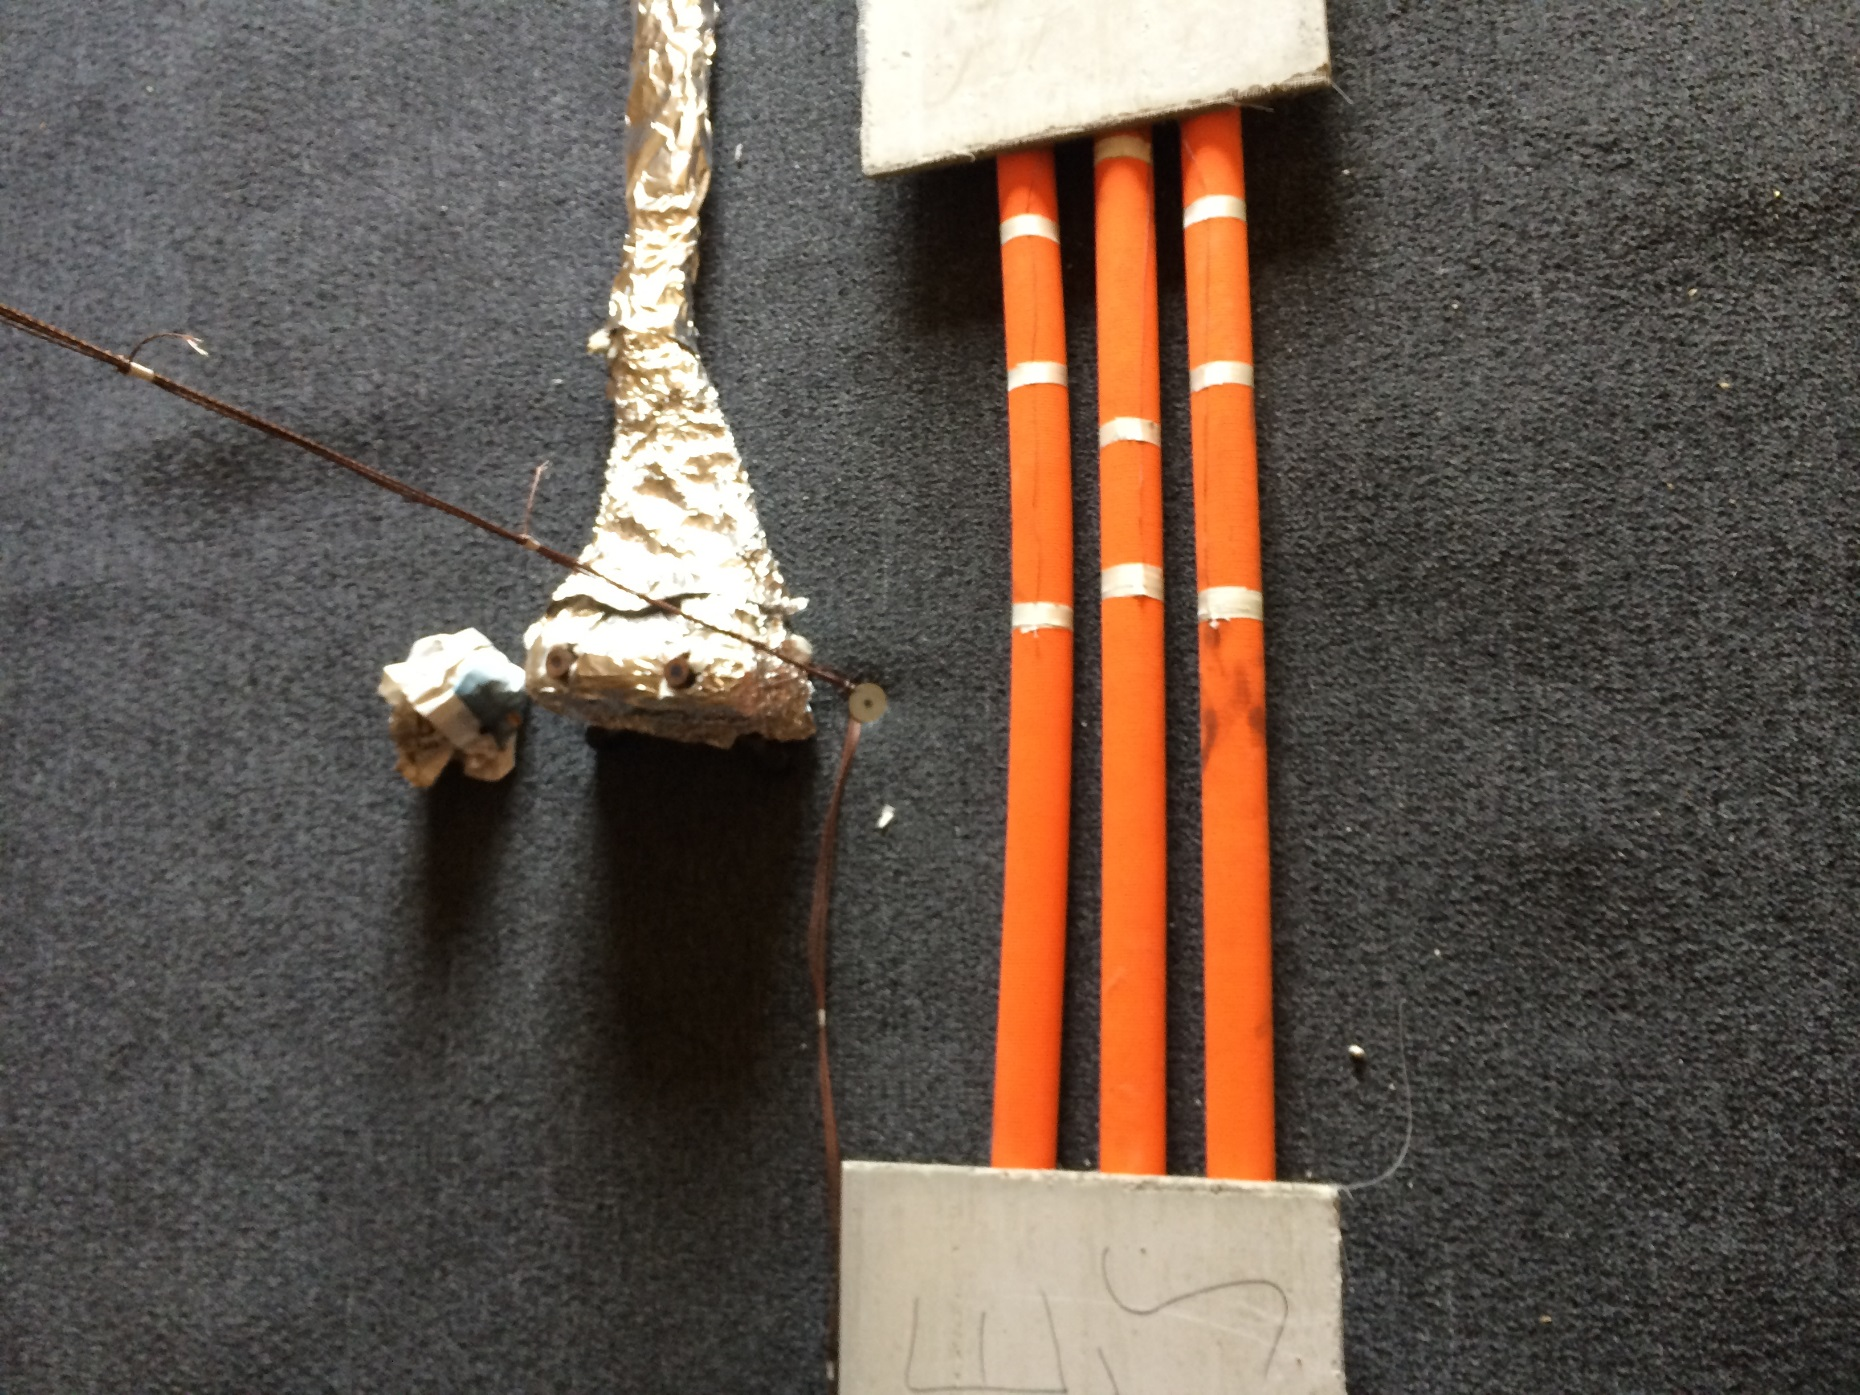
\includegraphics[width=0.8\columnwidth]{../Figures/Hose_Figures/test_setup_1b}
\caption{Locations of instrumented hose samples relative to the vertical thermocouple array, the heat flux gauge and the radiometer.}
\label{fig:test_setup_1b}
\end{figure}

\section{Hose}
The fire hose that was used for the experiments was ``Big - 10'' brand manufactured by Key Hose. According to the manufacturer the hose meets or exceeds all of the performance requirements of NFPA 1961. The ``1 3/4"~in. hose is constructed with 100 polyester double jacket and the rubber lining is made of a single-ply extruded tube of synthetic EPDM a minimum wall thickness of 0.040~in. The hose condition was new, right out of the box. See Attachment 1 for further hose information.

\begin{figure}[!ht]
\centering
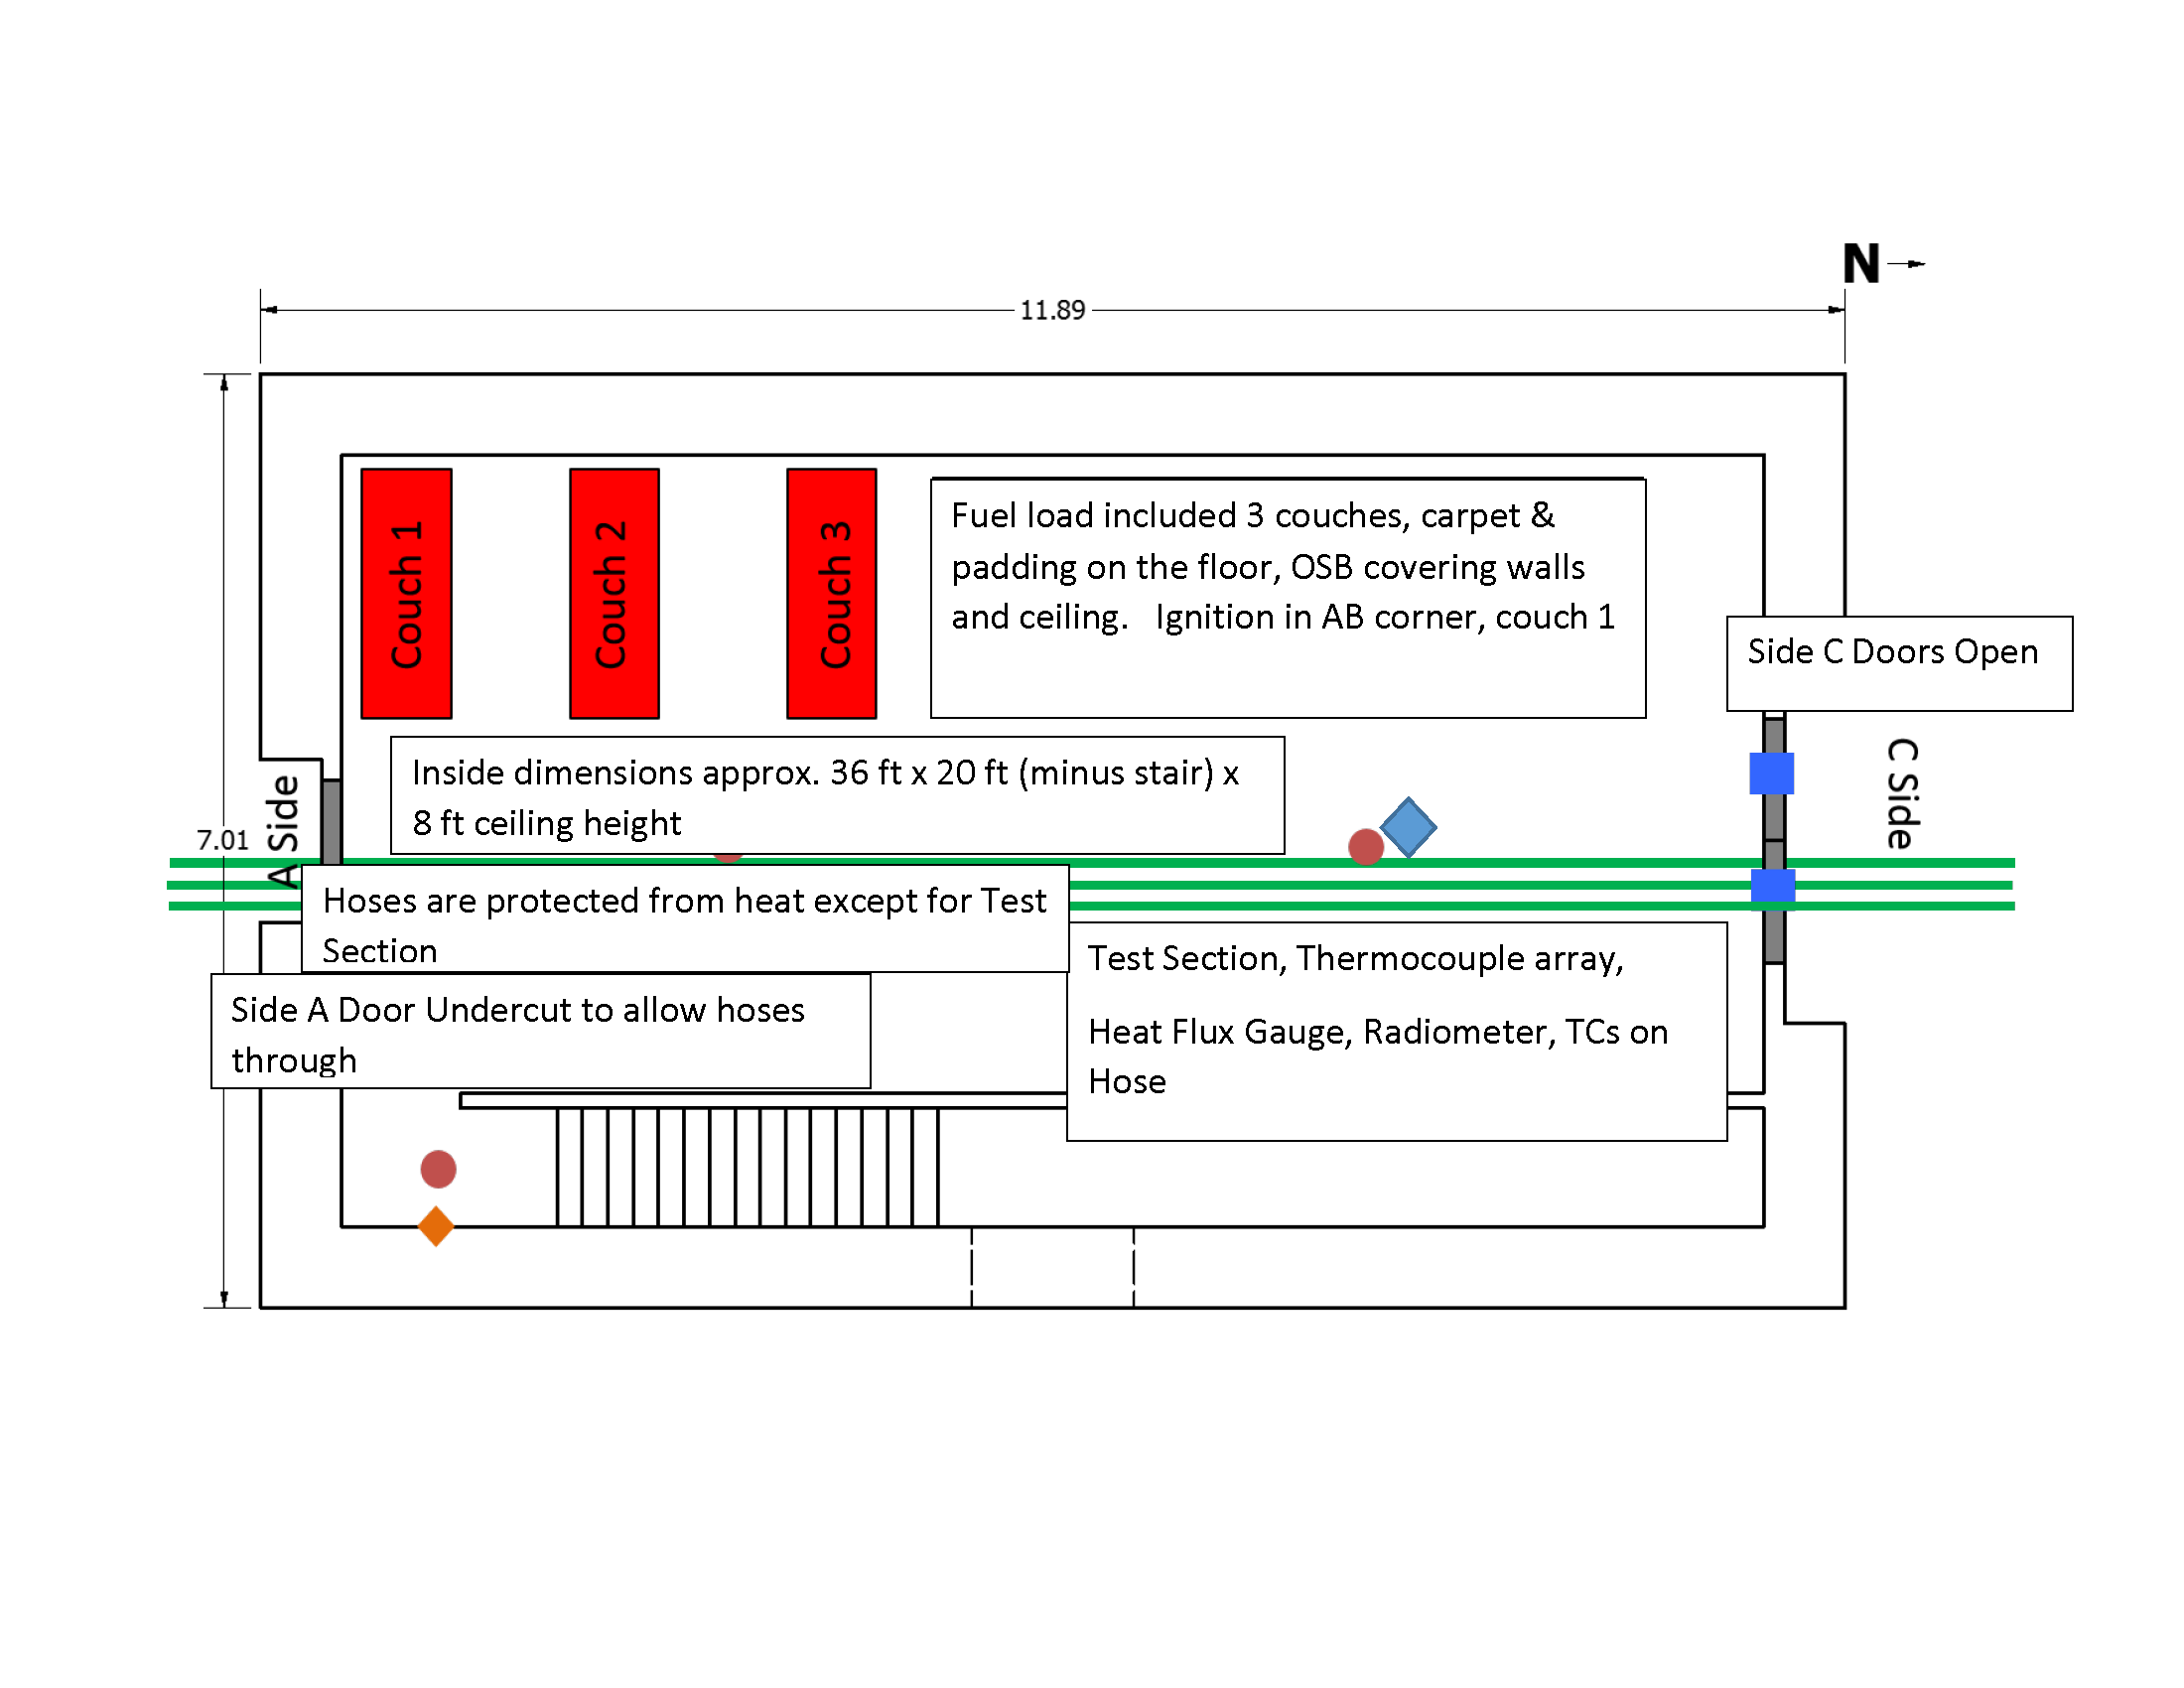
\includegraphics[width=.8\columnwidth]{../Figures/Hose_Figures/test_plan}
\caption{Schematic showing the test arrangement on the lower level. The circle represents the thermocouple array, the diamond represents the heat flux gauge and radiometer, and the squares represent the bi-directional velocity probes in the open doorway on Side C.}
\label{fig:test_plan}
\end{figure}

\section{Results}
Two experiments were conducted to examine the amount of thermal exposure required to cause the fire hose to burn through. In each experiment three different hose conditions were examined: hose filled with air, hose filled with water, hose flowing 150 gpm of water. The difference between the two experiments was the location of the exposed hose section. In Experiment 1 the center of the exposed hose section and instrumentation was located 11 ft from the open doorway on Side C. In Experiment 2 the exposed hose section and instrumentation was located 4~ft from the open doorway on Side C.  

In Experiment 1, all three hose samples failed during the transition to flashover. Given the high rate of change of the thermal exposure in Experiment 1, the exposed section was moved closer to the open doorway for Experiment 2 as an attempt to reduce the exposure by taking advantage of the cool air being entrained near the floor through the open door way. In Experiment 2, the hose filled with air failed followed by the hose filled with static water.  These two ruptures happened very close together in time. The water from the ruptured line suppressed the fire to a degree and protected the hose line with the flowing water, so that it did not fail although the outer jacket was burned away and the hose was compromised.

\begin{figure}[!ht]
\centering
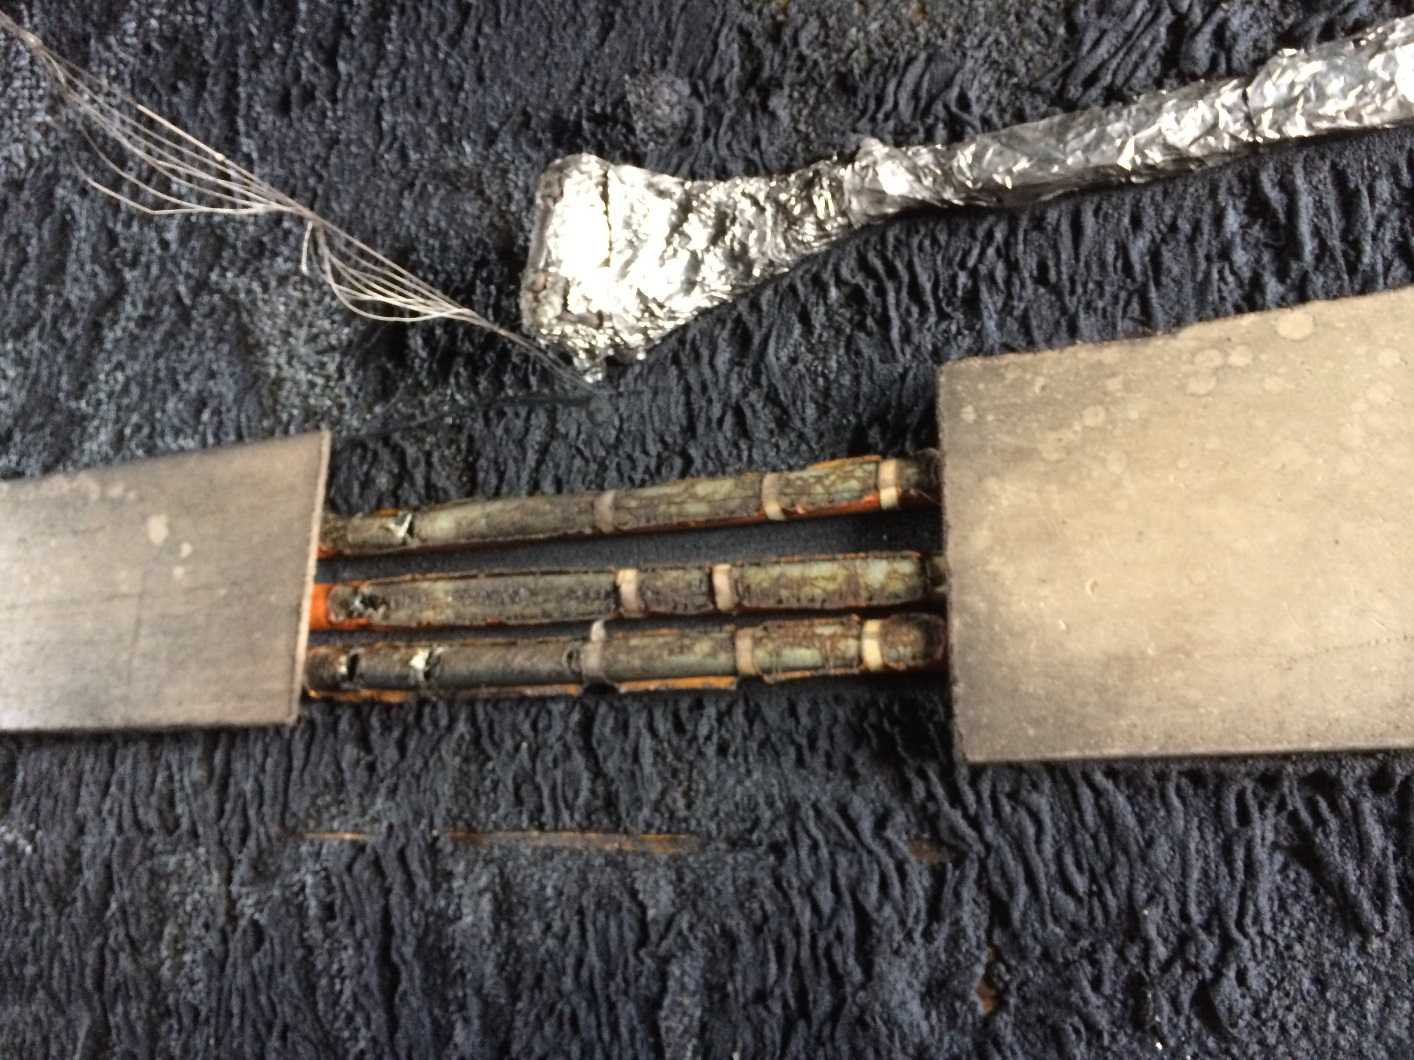
\includegraphics[width=.8\columnwidth]{../Figures/Hose_Figures/hose_post_exp1}
\caption{Photograph after Experiment 1. All three hoses burned through within 2 seconds of each other. The hose at the top of the photograph was the static water line.  The middle hose was filled with air. The lower hose is the hose that was flowing 150~gpm of water.}
\label{fig:post_test1_image}
\end{figure}

\begin{figure}[!ht]
\centering
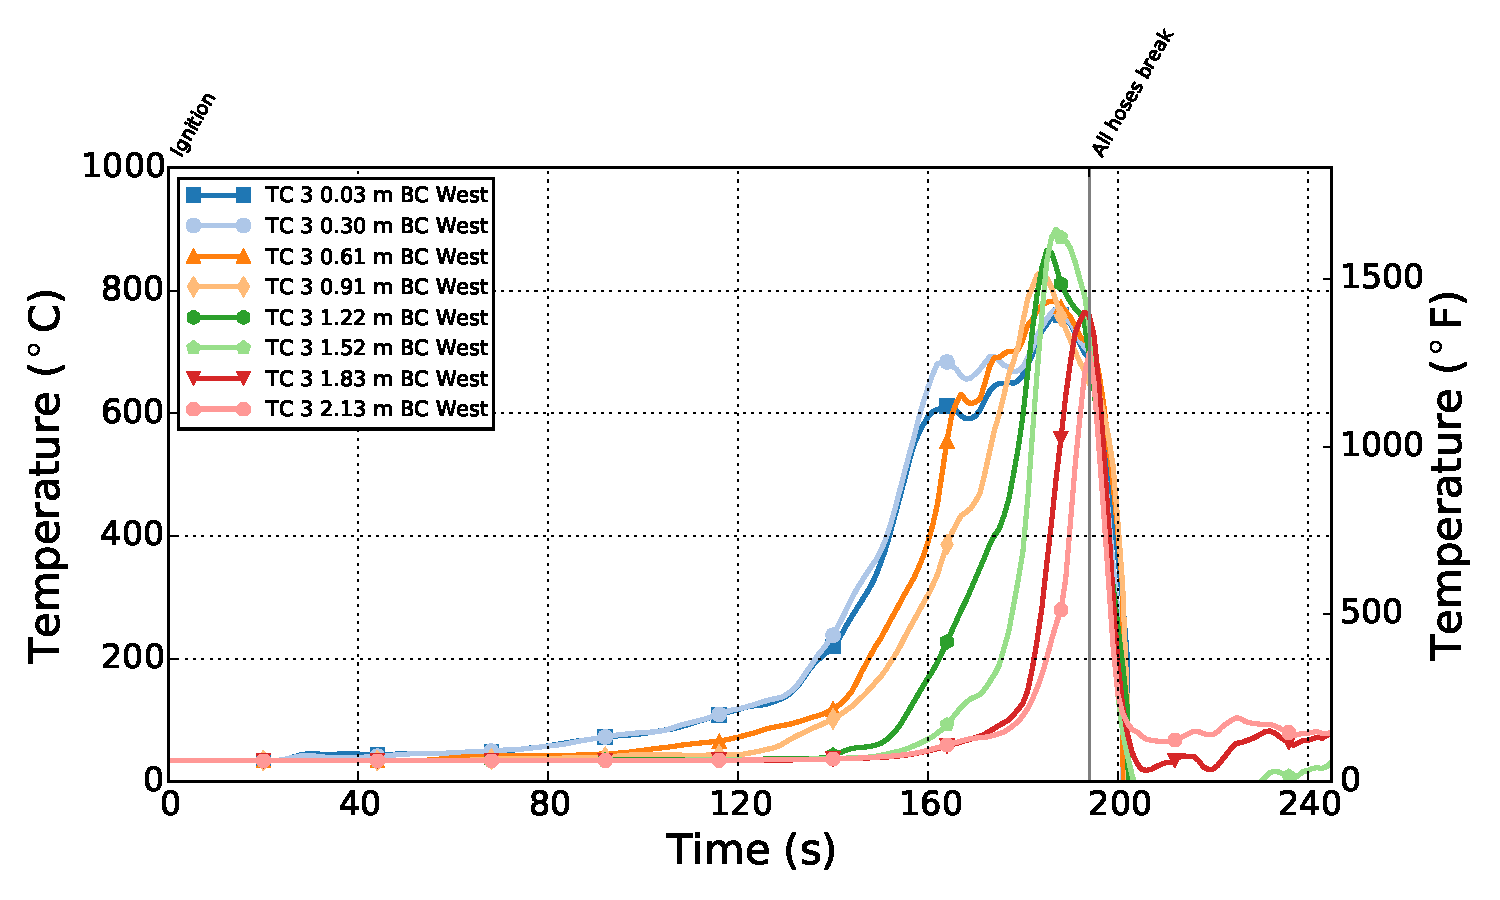
\includegraphics[width=\columnwidth]{../Figures/Hose_Figures/Test_60_West_80915_TC_A3}
\caption{Thermocouple temperatures as a function of elevation at the test section for Experiment 1.}
\label{fig:temp_A3_test60}
\end{figure}

\begin{figure}[!ht]
\centering
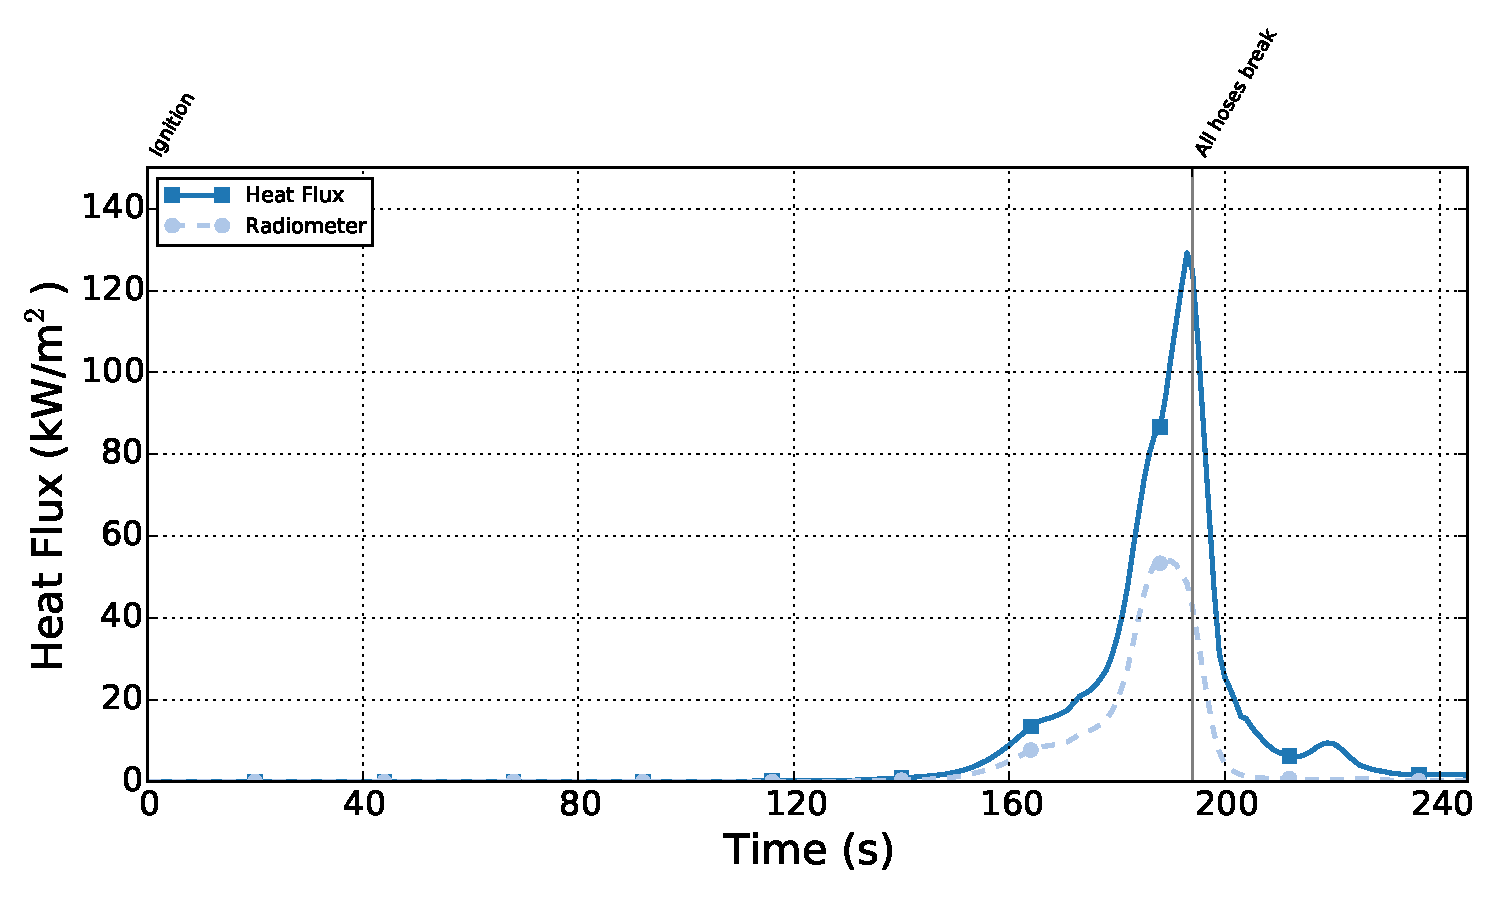
\includegraphics[width=\columnwidth]{../Figures/Hose_Figures/Test_60_West_80915_Heat_Flux_2}
\caption{Total and radiant heat flux at the test section for Experiment 1.}
\label{fig:hf_A3_test60}
\end{figure}

\begin{figure}[!ht]
\centering
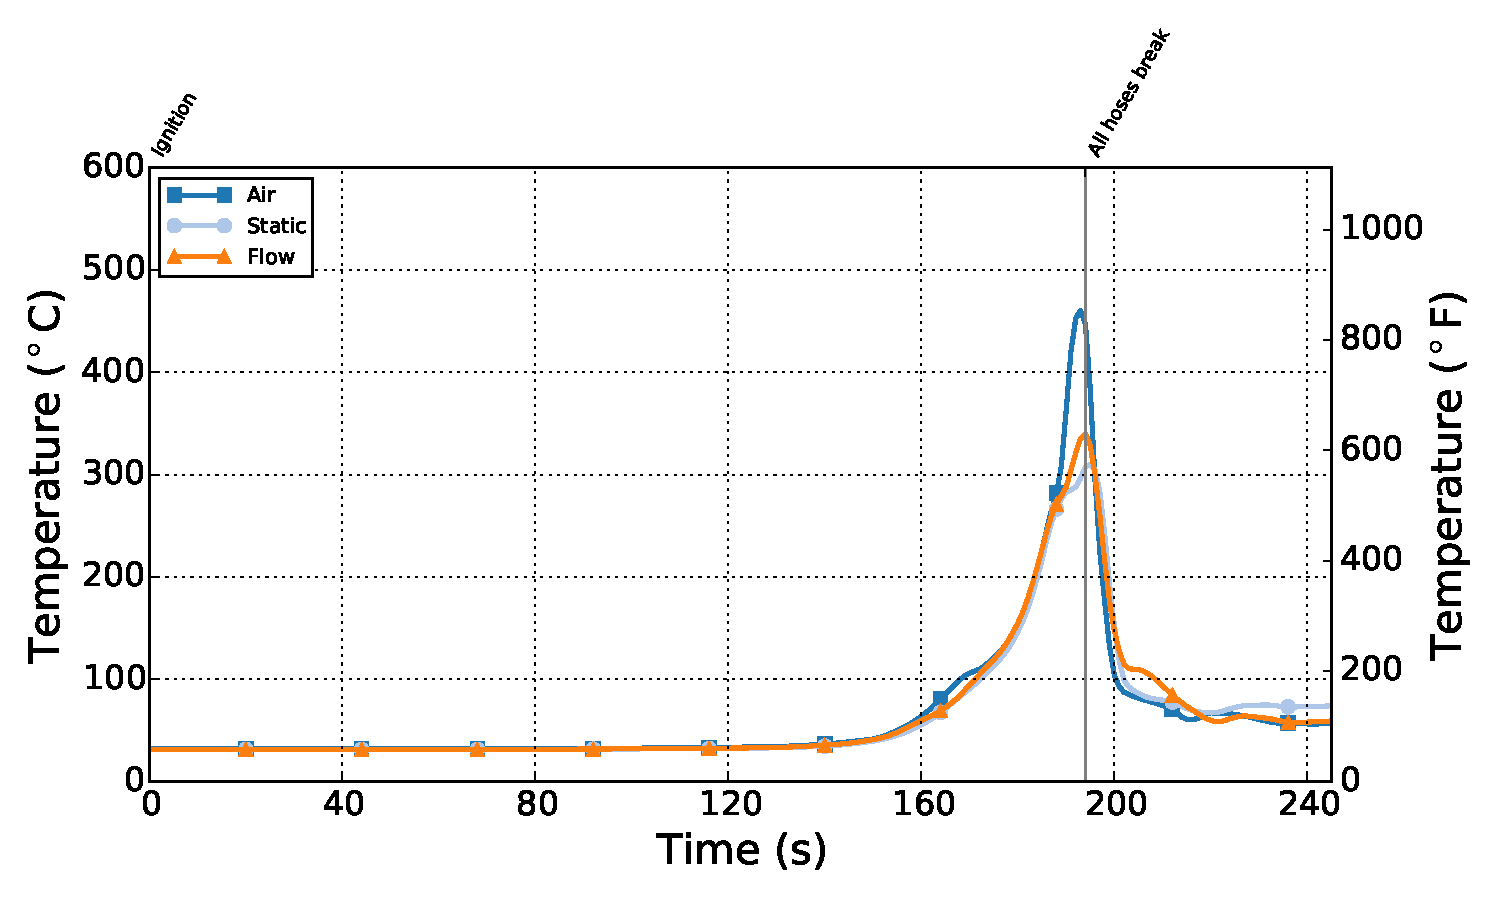
\includegraphics[width=\columnwidth]{../Figures/Hose_Figures/Test_60_West_80915_TC_Gear_2}
\caption{Thermocouple temperatures at the test section for each hose tested for Experiment 1.}
\label{fig:hose_A3_test60}
\end{figure}

\begin{figure}[!ht]
\centering
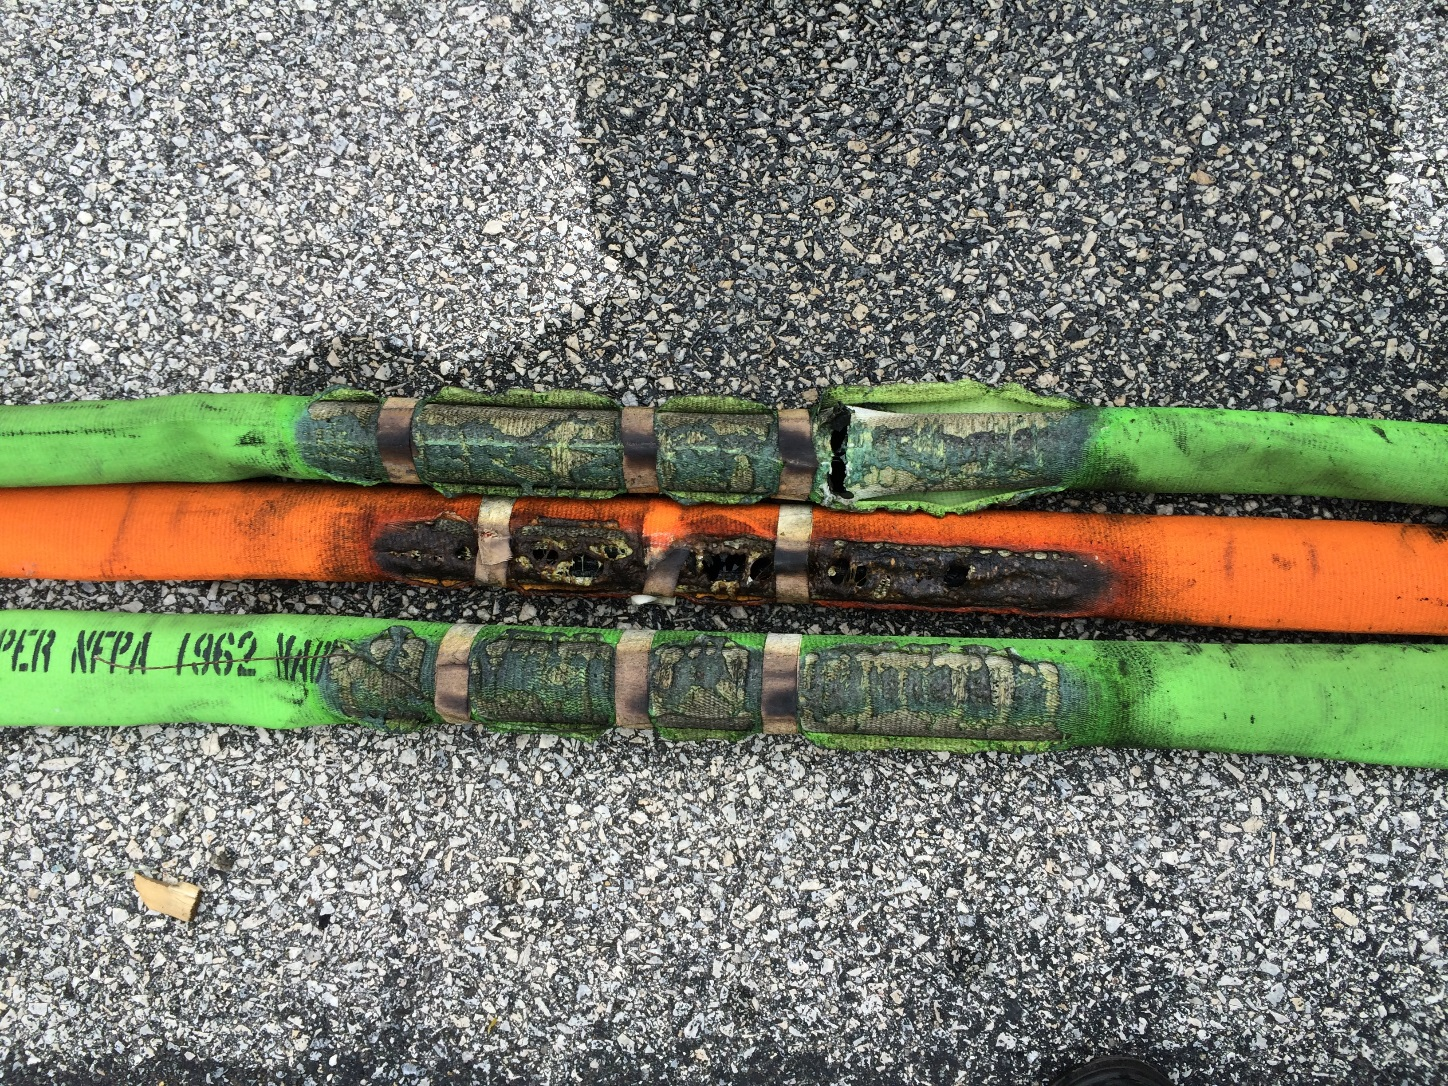
\includegraphics[width=.8\columnwidth]{../Figures/Hose_Figures/hose_post_exp2}
\caption{Photograph showing the damage to the hose samples after Experiment 2. The hose at the top of the photograph was the static water line. The middle hose was filled with air. The lower hose is the hose that was flowing 150~gpm of water.}
\label{fig:post_test2_image}
\end{figure}

\begin{figure}[!ht]
\centering
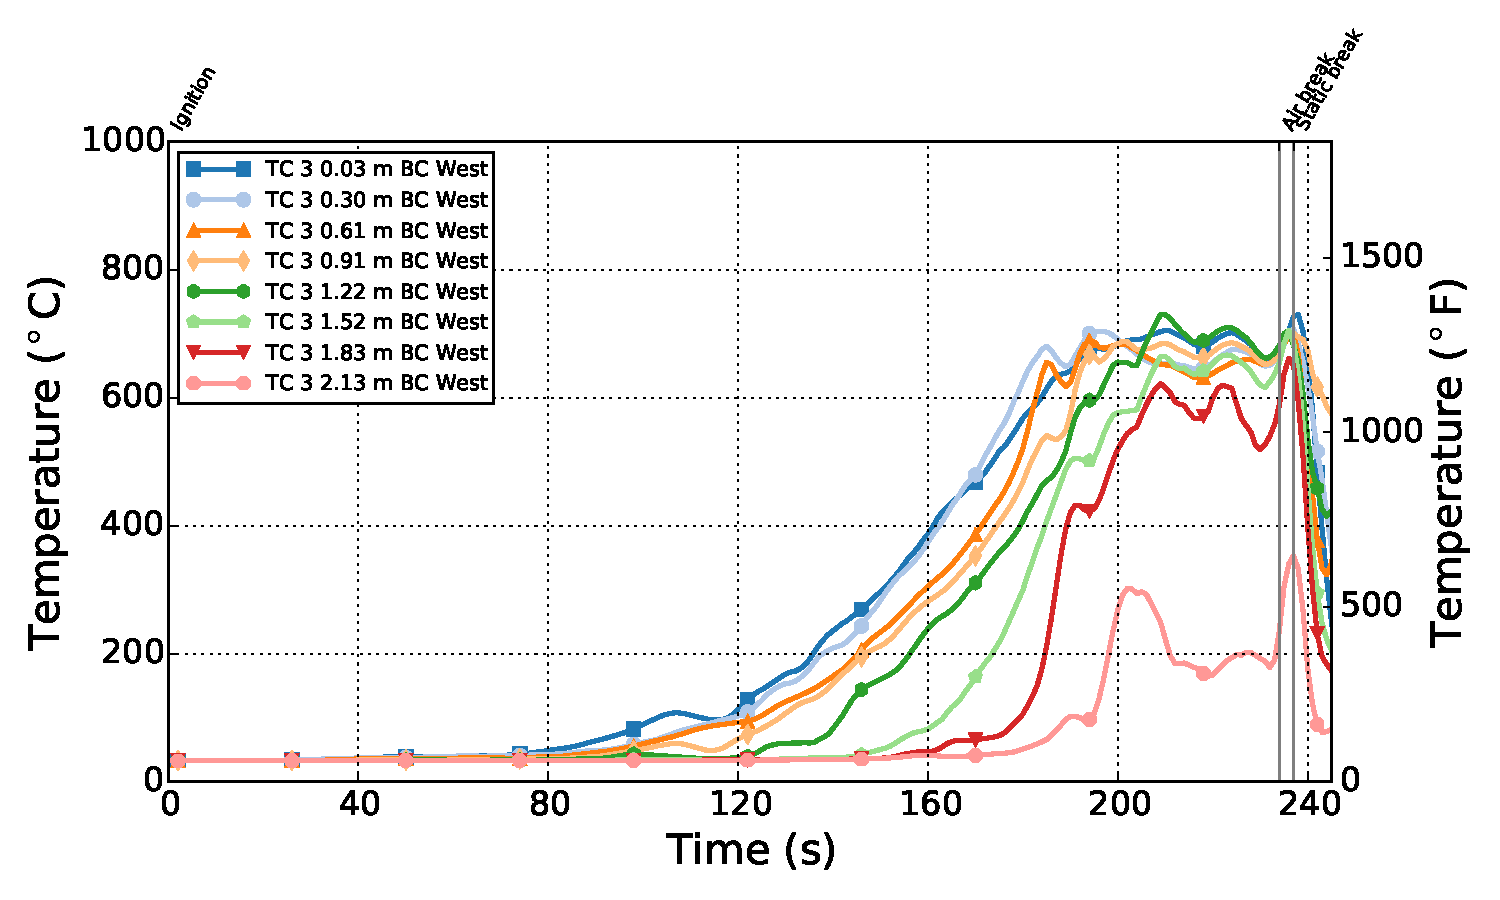
\includegraphics[width=\columnwidth]{../Figures/Hose_Figures/Test_62_West_81015_TC_A3}
\caption{Thermocouple temperatures as a function of elevation at the test section for Experiment 2.}
\label{fig:temp_A3_test62}
\end{figure}

\begin{figure}[!ht]
\centering
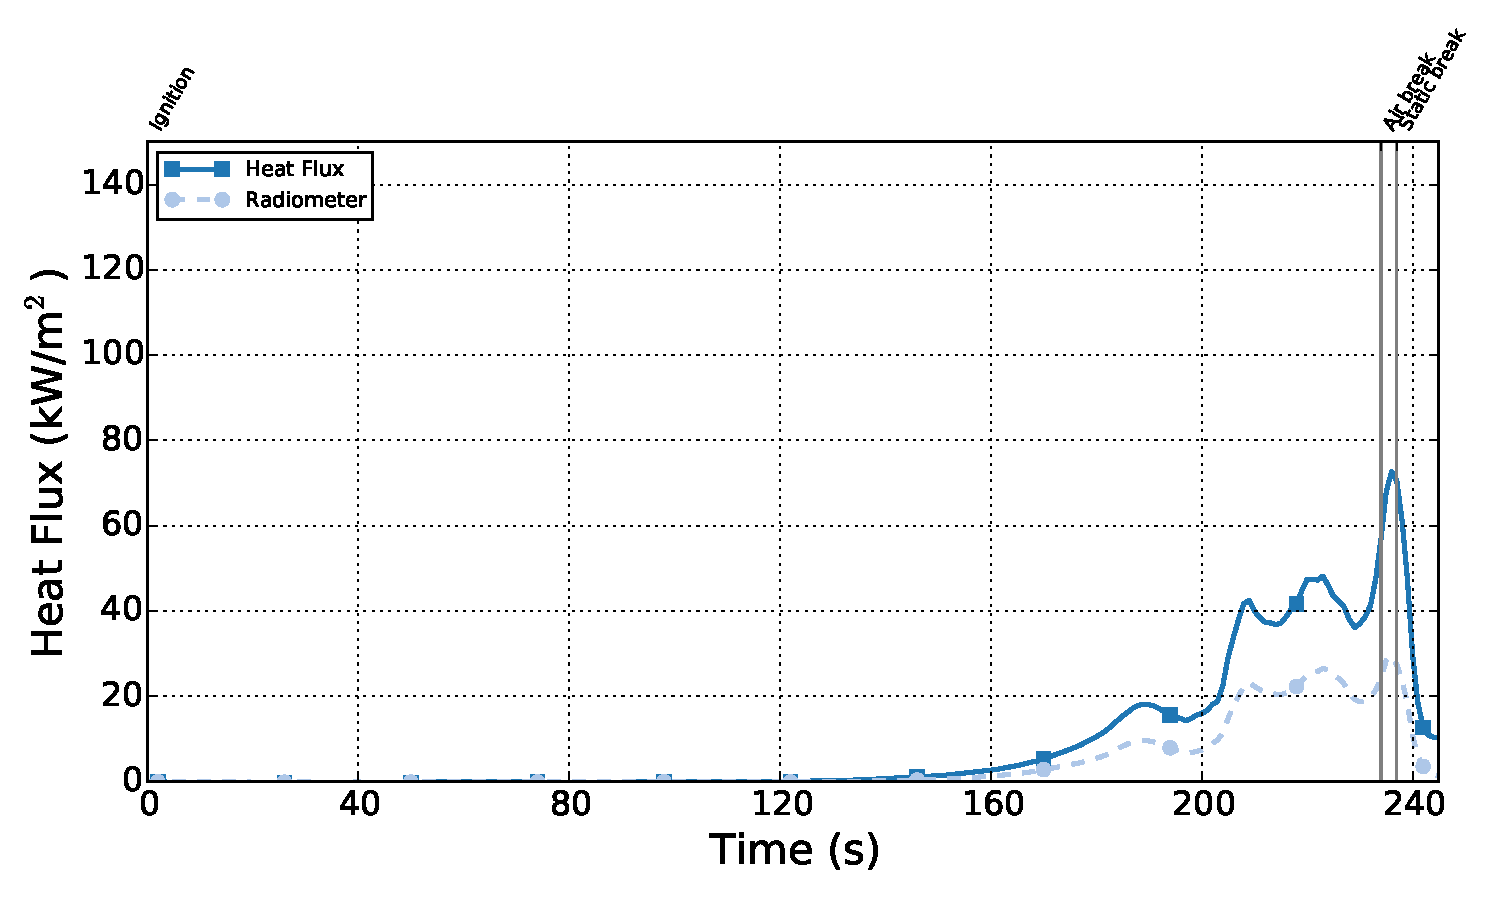
\includegraphics[width=\columnwidth]{../Figures/Hose_Figures/Test_62_West_81015_Heat_Flux_2}
\caption{Total and radiant heat flux at the test section for Experiment 2.}
\label{fig:hf_A3_test62}
\end{figure}

\begin{figure}[!ht]
\centering
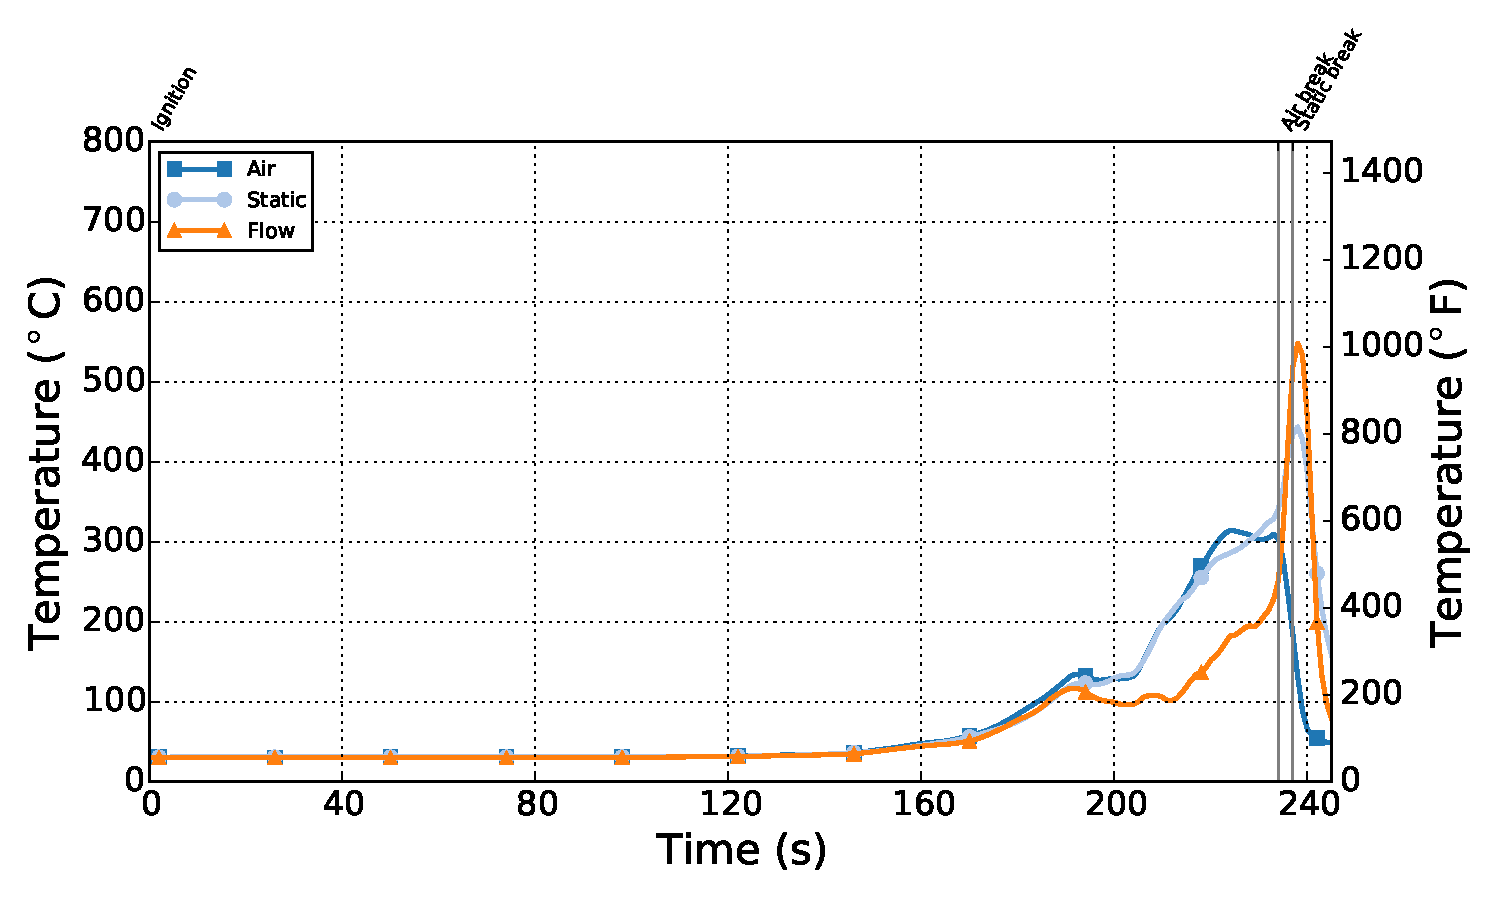
\includegraphics[width=\columnwidth]{../Figures/Hose_Figures/Test_62_West_81015_TC_Gear_2}
\caption{Thermocouple temperatures at the test section for each hose tested for Experiment 2.}
\label{fig:hose_A3_test62}
\end{figure}

\section{Summary}
These two experiments provide some insight in the level of energy required to burn through a hose. In both experiments, flames appeared to be close to the hose, if not impinging on the hose at the time of burn through. In these experiments there was no significant difference in burn through time for the hoses filled with air, static water or flowing water.   


%----------------------------------------------------------------------------------------

\end{document}